\documentclass[conference]{IEEEtran}

\usepackage{cite}
\usepackage{amsmath,amssymb}
\usepackage{graphicx}
\usepackage{booktabs}
\usepackage{tikz}
\usepackage{xcolor}
\usepackage{hyperref}
\usepackage{pgfplots}
\pgfplotsset{compat=newest}

\hypersetup{
    colorlinks=true,
    linkcolor=blue,
    citecolor=blue,
    urlcolor=blue
}

\begin{document}

\title{Historical Case Study on Ti Silicide (TiSi\textsubscript{2}) \\ Reliability Issues in Legacy CMOS Nodes}

\author{
\IEEEauthorblockN{Shinichi Samizo}
\IEEEauthorblockA{Independent Semiconductor Researcher\\
Project Design Hub, Samizo-AITL\\
\textit{Email:} \href{mailto:shin3t72@gmail.com}{shin3t72@gmail.com}\quad
\textit{GitHub:} \href{https://github.com/Samizo-AITL}{Samizo-AITL}}
}

\maketitle

\begin{abstract}
This paper analyzes a historical failure case related to Ti silicide (TiSi\textsubscript{2}) phase transition instability at the 0.25~µm CMOS node. 
The incomplete C49$\rightarrow$C54 transformation, coupled with boron absorption, caused localized high-resistance spots that directly reduced SRAM yield. 
The case illustrates how process optimization and empirical feedback cycles became indispensable in semiconductor development, particularly when economic pressure and high-voltage compatibility shaped process selection.
\end{abstract}

\section{Introduction}
In the late 1990s, LCD drivers for passive monochrome panels were commonly fabricated in 0.35~µm nodes supporting 3.3~V logic and 40~V high-voltage transistors.  
With the transition to active-matrix TFT (aTFT) color panels in the early 2000s, demand increased for higher-performance logic and embedded SRAM, along with high-voltage device integration.  

Although the 0.18~µm process was already in mass production and offered smaller chip size and stable yield, it relied on shallow trench isolation (STI). STI edge thinning posed risks for 30~V device reliability.  
By contrast, the 0.25~µm process used local oxidation of silicon (LOCOS), which had a proven track record in high-voltage isolation.  
Therefore, manufacturers adopted the 0.25~µm LOCOS process (3.3~V + 30~V) for LCD driver ICs despite disadvantages in chip area.

\begin{table}[!t]
\centering
\caption{Comparison of 0.25~µm (LOCOS) vs 0.18~µm (STI) nodes}
\begin{tabular}{@{}lll@{}}
\toprule
 & 0.25~µm (LOCOS) & 0.18~µm (STI) \\ \midrule
Isolation method & LOCOS (thick field oxide) & STI (trench oxide) \\
HV support & Proven 30~V & Edge thinning risk at 30~V \\
Chip size & Larger & Smaller \\
Yield stability & Moderate (silicide risk) & Generally stable \\
Adoption reason & Safe HV integration & Not adopted for HV products \\ \bottomrule
\end{tabular}
\label{tab:process_comparison}
\end{table}

\section{Technical Background}
TiSi\textsubscript{2} was widely adopted for its low resistivity. 
However, the silicide undergoes a phase transition from metastable C49 to stable C54 during rapid thermal annealing (RTA). 
If the transition is incomplete, residual C49 grains act as high-resistance regions. 
Furthermore, boron absorption into TiSi\textsubscript{2} aggravated resistance fluctuation, directly manifesting as random SRAM bit failures.

\section{Failure Analysis}
In early products embedding 500k-bit SRAM macros, the instability did not critically manifest.  
However, with 1M-bit macros, single-bit failures became frequent due to localized high-resistance spots in transistor contact regions.  
Because no redundancy was included, each defect directly caused chip rejection.  
At the development review stage, these issues were not anticipated, as empirical data from smaller SRAM macros suggested acceptable yield.

\begin{figure}[!t]
  \centering
  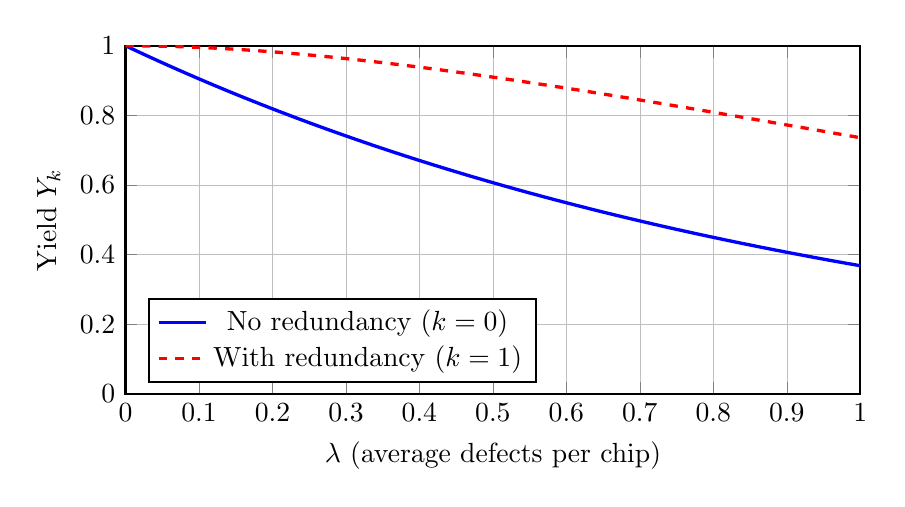
\begin{tikzpicture}
    \begin{axis}[
      width=0.9\linewidth,
      height=6cm,
      xlabel={$\lambda$ (average defects per chip)},
      ylabel={Yield $Y_k$},
      xmin=0, xmax=1,
      ymin=0, ymax=1,
      legend pos=south west,
      grid=both,
      major grid style={line width=.2pt,draw=gray!50},
      minor grid style={line width=.1pt,draw=gray!20},
      thick,
    ]
      \addplot[blue, very thick, domain=0:1, samples=200] {exp(-x)};
      \addlegendentry{No redundancy ($k=0$)}

      \addplot[red, dashed, very thick, domain=0:1, samples=200] {exp(-x)*(1+x)};
      \addlegendentry{With redundancy ($k=1$)}
    \end{axis}
  \end{tikzpicture}
  \caption{Illustrative yield sensitivity (Poisson model) with and without redundancy.}
  \label{fig:yield}
\end{figure}

\section{Design Review Limitations}
Design reviews (DR) primarily checked rule compliance and did not evaluate risks arising from incomplete silicide transformation.  
Since prior SRAM macros (≤500k bits) had not shown systematic failure, extrapolation to 1M-bit macros appeared reasonable but proved incorrect.  

\section{Countermeasures}
\subsection{Provisional Measures}
Etch profiles were adjusted to slightly undercut sidewalls, ensuring sufficient separation between halo implants and active regions.  
This temporarily improved yield.

\subsection{Permanent Measures}
RTA conditions were optimized to stabilize C54 phase formation.  
However, this altered device parameters, requiring re-characterization of process-device models.

\section{Educational Application}
\subsection{Teaching Materials}
\begin{itemize}
    \item Cause-effect diagrams (process $\rightarrow$ defect $\rightarrow$ yield)
    \item Comparative table: 0.25~µm (LOCOS) vs 0.18~µm (STI) for HV devices
    \item Exercises: prioritize process fix vs introduce redundancy
\end{itemize}

\subsection{Universality}
The trade-off was not merely cost vs. stability but meeting the integration requirements of active-matrix LCD drivers: high-performance logic, large SRAM, and safe HV operation.  
Such process-selection dilemmas remain relevant in later nodes (e.g., 28~nm FD-SOI reuse, 40~nm BCD continuity).

\section{Conclusion}
This case demonstrates how the need for HV compatibility constrained process selection, leading to the adoption of 0.25~µm LOCOS despite the availability of a smaller, stable 0.18~µm STI process.  
Yield degradation from incomplete TiSi\textsubscript{2} phase transition highlighted the necessity of empirical feedback cycles in design and process development.  
Its educational value lies in using historical semiconductor case studies to teach the interaction of technology, reliability, and market context.

\section*{References}
\begin{thebibliography}{99}
\bibitem{Sze2007} S. M. Sze and K. K. Ng, \textit{Physics of Semiconductor Devices}, 3rd ed. Wiley, 2007.
\bibitem{Wolf1986} S. Wolf and R. N. Tauber, \textit{Silicon Processing for the VLSI Era, Volume 1: Process Technology}. Lattice Press, 1986.
\bibitem{Colinge2004} J.-P. Colinge, \textit{Silicon-on-Insulator Technology: Materials to VLSI}, 3rd ed. Springer, 2004.
\bibitem{ITRS2001} International Technology Roadmap for Semiconductors (ITRS), ``Process Integration, Devices, and Structures,'' 2001.
\bibitem{Takeda1994} E. Takeda, C. Y. Yang, and A. S. Grove, ``Silicide technology for ULSI applications,'' \textit{IEEE Trans. Electron Devices}, vol. 41, no. 12, pp. 2133--2141, Dec. 1994.
\bibitem{Chang1996} J. P. Chang and A. J. Steckl, ``Titanium silicide formation and stability in submicron CMOS technology,'' \textit{J. Appl. Phys.}, vol. 79, no. 9, pp. 4536--4364, 1996.
\end{thebibliography}

\section*{Author Biography}
\textbf{Shinichi Samizo} received the M.S. degree in Electrical and Electronic Engineering from Shinshu University, Japan.  
He worked at Seiko Epson Corporation on semiconductor memory and mixed-signal device development and contributed to inkjet MEMS actuators and PrecisionCore printhead technology.  
He is currently an independent semiconductor researcher focusing on process/device education, memory architecture, and AI system integration.\\
\emph{Contact:} \href{mailto:shin3t72@gmail.com}{shin3t72@gmail.com}\quad
\emph{GitHub:} \href{https://github.com/Samizo-AITL}{Samizo-AITL}.

\end{document}
